% !TEX root = /Users/royc/Google_Drive/Thesis/RoyC_Umass_Thesis.tex
\chapter{Introduction}  \label{Intro} 
\lhead{Chapter 1. \emph{Introduction}} 
%----------------------------------------------------------------------------------------
\section{Fixed Genomes and Flexible Genes}
  \label{Intro:sec:Fixed Genomes and Flexible Genes} 

  Exodus tells of the liberation of the Israelites from Egyptian slavery. Humble and reluctant Moses, their divine-appointed leader, attempts to force the Pharaoh Ramses to release the Israelites through inflicting 10 plagues. Pharaoh is stalwart and stubborn as water turns to blood, streets are flooded with frogs, lice, and flies. As livestock falls dead from disease, people and animals both are covered in boils, and the land burns in storms of fire, Pharaoh does not bend.

  The 8th plague was a swarm of Locusts, described in Exodus 10: 14-15:

  \begin{quote}
    \itshape
    \singlespacing
    \textsuperscript{14} And the locusts went up over all the land of Egypt, and rested in all the coasts of Egypt: very grievous were they; before them there were no such locusts as they, neither after them shall be such.\\ 
      \\
    \textsuperscript{15} For they covered the face of the whole earth, so that the land was darkened; and they did eat every herb of the land, and all the fruit of the trees which the hail had left: and there remained not any green thing in the trees, or in the herbs of the field, through all the land of Egypt.
    \end{quote}

  The desolation of a locust plague was still not enough to persuade Ramses. Nor three days of darkness. Only the death of all first-born Egyptians, included Ramses own son, was enough to persuade Pharaoh to liberate the Israelites.

  Locust swarms are not biblical fantasy. It is perhaps the most \textit{believable} of the 10 plagues. Today the United Nations' Food and Agriculture division maintains a \href{http://www.fao.org/ag/locusts/en/info/info/news/index.html}{Locust watch website} that provides weekly updates on potential swarms in northern Africa and the Middle East. Locusts have long been, and continue to be, a powerful and feared force of Nature.

  Unlike fire and brimstone, locusts are something that can be observed and studied. What triggers a swam? We know that the desert locust, \locusts{}, is the one of 10 species that swarm and cause massive crop damage. \locusts{} are in the insect Order Orthoptera, along with crickets and katydids. Orthoptern members make sound known as \textit{stridulation} by vigorously rubbing their wings, making for a noisy cloud of devastation. Desert Locusts only weigh 0.05-- 0.07 ounces, and are less than 2.5 inches long. They consume their own body weight in vegetation per day. One \href{http://animaldiversity.ummz.umich.edu/site/accounts/information/Melanoplus_spretus.html}{swarm} of the infamous, and now curiously extinct, Rocky Mountain locust contained 12.2 \textit{trillion} insects. Its estimated total weight was 27.5 million tons. The swarm covered almost 200 square miles (2/3 the size of Manhattan), and could travel 60 miles in a day. A locust swarm is truly a modern biblical plague.

  \begin{figure} % Desert Locus Figure
    \centering 
    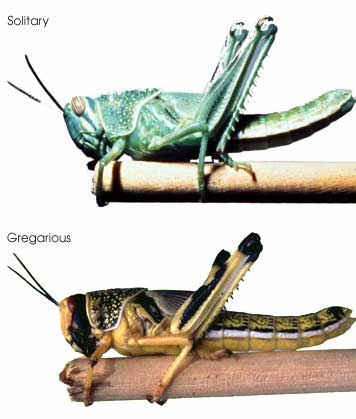
\includegraphics[width=10cm,keepaspectratio]{Figures/Intro/DesertLocust.jpeg}
    \caption[The Solitary and Gregarious forms of \locusts{}]
    {
      The Solitary and Gregarious forms of \locusts{}\\[0.25cm]
      The two phenotypic forms of \locusts{} appear very different. The Solitary form is green and generally larger, while its gregarious form is more brightly colored, smaller, and capable of swarming in vast numbers, destroying crops and vegetation. Photo from \href{http://www.wikicommons.com}{Wikicommons}.
      }
    \label{Intro:fig:Locust}
    \end{figure}

  By definition swarms are temporary; the movement, en masse, from one location to another. But where do 12.2 trillion locusts go when not swarming? Does anyone care if their crops aren't under assault? It seemed no one cared enough, until about 1921, when an important realization was made.

  The power and destruction \locusts{} can inflict makes it difficult to believe that they are nothing more than common grasshoppers. Nothing more than grasshoppers not just by analogy, but by actual \textit{Taxonomy}. Desert locusts are actually the \textit{gregarious} form  of \locusts{} (See Figure \ref{Intro:fig:Locust}), while the more familiar and docile looking ``grasshopper'' is the \textit{solitary form}. How does such a dichotomy to exist within the same organism, indeed the same \textit{genome}?

  \locusts{} are \textit{polyphenic}, meaning that they have multiple (poly) physical forms (phenotypes). Polyphenism is a general feature among insects. These phenotypes are often extremely different. For example, pea aphids (\textit{Acyrthosiphon pisum}), which usually exist in an asexually reproducing, wingless female form, respond to reduced food supply and overcrowding by producing winged offspring. Winged organisms travel to new sources of food and revert back to the asexually reproducing form \citep{Shingleton2003,Purandare2014b}. In the case of \locusts{}, the gregarious form is smaller and more brightly colored compared to its solitary cousins. This transformation can happen in as little as two hours. What is the underlying cause of this transformation?

  In 2009, \citet{Anstey2009} reported that after two hours of forced crowding \locusts{} displayed elevated levels of the neurotransmitter serotonin in the ganglia (brain). Serotonin levels were strongly correlated with other gregarious form indicators. Serotonin regulates neuronal junctions and wiring in the brain \citep{Hoeffer2003}. Through the integration of environmental and social cues, the grasshopper brain can be re-wired, resulting in tremendous changes in behavior and phenotype. These changes prepare the organism to deal with a different world and allows the species to survive. This survival is to the detriment of surrounding agriculture.

  In an extremely interesting \href{http://aeon.co/magazine/nature-and-cosmos/why-its-time-to-lay-the-selfish-gene-to-rest/}{article}, David Dobbs compares the two forms of \locusts{} to that of Dr Jekyll and Mr. Hyde, the principle characters of in the Robert Louis Stevenson novella. For Dr Jekyll in fiction, and for \locusts{} in reality, the power to morph into multiple forms demonstrates the incredible power of a fixed genome yet plastic gene expression. 

  It is often said that something is ``in the genes.'' Another oft-heard idiom that is perhaps more more appropriate is: ``it's how you use them.'' This thesis will illustrate that, with ever increasing resolution in the measurement of functional gene products (i.e. the ``transcriptome''), we are just now beginning to appreciate the tremendous diversity and complexity of gene expression.

\section{Nucleic Acid Sequencing}
  \label{Intro:sec:Nucleic Acid Sequencing}

  \subsection{DNA Sequencing History}
    \label{Intro:subsec:DNA Sequencing History}

    Soon after it was realized that DNA is the source of genetic information in all living organisms \citep{Watson1953a}, and the \textit{pretty} and \textit{elegant} arrangement of complementary, antiparrallel, DNA strands was known \citep{Watson2012a}, the ability to determine specific arrangements of nucleotide bases (i.e. to ``sequence'') in a given length of DNA was seen as a critical missing piece of technology. It took 25 years after the structure of DNA was known to be able sequence it. By 1977, two completely different methods developed by Sanger \citep{Sanger1975a,Sanger1977b} and Maxam-Gilbert \citep{Maxam1977a} were reported. These sequencing technologies, from then on referred to eponymously as ``Sanger'' or ``Maxam-Gilbert'' sequencing, were used to determine the specific order of a small piece of DNA (200-300 nt). Sanger sequencing soon dominated most sequencing reactions, likely due to the conceptually more intuitive nature of the technology. Over the next 35 years, DNA sequences were slowly cloned, sequenced, analyzed, and dutifully cataloged into knowledge.

    During the late 1970's and throughout the 1980's, DNA sequences were typically communicated in important publications \citep{Cordell1980a,Sanger1978a}. The birth of the Internet in the 1990's allowed publically-funded repositories for sequence information \citep{Benson2011a}. The human genome project \citep{Lander2011a,Venter2001}, provided the important activation energy that brought DNA sequencing from a hard-to-perform, but necessary, analysis, to an organized large-scale effort of assembling the complete genetic material complex genomes. An often criticized, but undeniably disrupting force in the human genome project was the competing efforts of the privately-owned company Celera \citep{Venter2008a}. Taking a higher-throughput and centralized approach to determining the sequence of the human genome, Celera fundamentally changed the landscape of genome assembly. Instead of assigning specific sections of the genome to be worked out by individual labs, Celera parallelized the effort. Celera collected the best ``high-throughput'' Sanger-sequencing devices from Agilent (ABI 3700 DNA Analyzer) and used a ``shotgun'' approach \citep{Staden1979}, sequenced pairwise \citep{Roach1995}. Combined with sequence scaffolds made available by the publicly-funded project, Celera was able to assemble a high-quality genome very quickly. Arguably, this was the first deep sequencing effort. Coincident with the beginning of a new millennium, it forever changed the landscape of molecular and biochemical research.

  \subsection{History of High-throughput Sequencing}
    \label{Intro:subsec: History of HTS}

    Sequencing DNA by Sanger's technology remains a valuable and critical tool in every biological scientist's toolbox. However, Sanger sequencing has  a practical throughput limit. Each DNA molecule to be sequenced must be isolated and clonally amplified using bacteria. Given that the human genome \citep{Hattori2005a} comprises >3 billion bp, and each Sanger reaction provides \textasciitilde800 nt of quality sequence, at least \textasciitilde4 million individual reactions are needed to determine the sequence of the human genome. This number assumes all ``reads'' are of sufficient quality, length, and do not overlap by even 1 nt. The use of reads with no overlap is out of the question, as overlaps are essential for assembling individual sequences via overlaps, critical for assembly through repeated sequences. 

    Even the best practical improvements to Sanger work-flows could not bring the technology in-line with aspirations of analyzing many species and/or organisms. Yet, the early 2000's saw multiple efforts to improve the scale of DNA sequencing, first using MPSS \citep{Brenner2000a}, but perhaps more importantly, by Pyro- \citep{Ronaghi1998a} and Polony sequencing \citep{Shendure2005}. Both pyro- and polony sequencing utilize emulsion PCR \citep{Nakano2003a} for clonal amplification prior to sequencing, removing the bottleneck of bacterial cloning. In contrast to Sanger sequencing, where fluorescencethe signal from the last incorporated chain-terminating nucleotide is observed, pyrosequencing visualizes light given off by luciferase reacting with pyrophosphate (PPi), a by-product of nucleotide incorporation. This approach was later commercialized by 454 technologies. Polony sequencing involves a more complicated sequencing-by-ligation method, eventually commercialized by Applied Biosystems and branded as SOLiD sequencing. While both of these technologies provided valuable, high-throughput sequences, neither has been as successful as the approach commercialized by Solexa, now known as Illumina.

    Illumina sequencers use a sequencing-by-synthesis approach. After clonal amplification of DNA on a slide surface \citep{Bentley2008}, fluorescent nucleotides are visualized as they are incorporated into the growing DNA strand. Since 2006, iterations of the Illumina platform (eg. GE, GE-II(x), Hi-Seq, Hi-Seq 2500, Hi X) have demonstrated a steady and impressive increases in both read depth and length. On February 15th 2012, Illumina announced on its \href{http://blog.basespace.illumina.com/}{Basespace blog}, that they had sequenced a HapMap sample at 40X coverage, using the HiSeq 2500 platform and paired-end 100 nt reads in a single run. On January 14th, 2014, Illumina \href{http://bit.ly/PZpegZ}{announced} its HiSeq X system, the first platform to truly attain the mythical \$1,000 genome. These machines demonstrate that sequencing genomes is no longer the monumental endeavor it once was and that completely new experimental possibilities are a reality for life science researchers (see Figure \ref{Intro:fig:SeqCosts}).

    \begin{figure} % Sequence Costs over time
      \centering 
      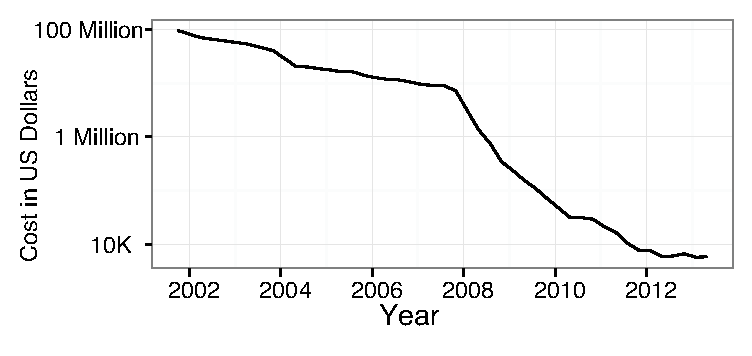
\includegraphics{Figures/Intro/Sequencing_costs_over_time.eps}
      \caption[Cost of sequencing the human genome over time]
      {
        Cost of sequencing the human genome over time\\[0.25cm]
        The costs of sequencing the human genome has decreased on a log scale over a roughly 10 year period thanks to major improvements in high-throughput sequencing. Data from Wetterstrand KA. DNA Sequencing Costs: Data from the NHGRI Genome Sequencing Program (GSP) Available at: \url{www.genome.gov/sequencingcosts}. Accessed 2013-09-03).
        }
      \label{Intro:fig:SeqCosts}
      \end{figure}

  \subsection{Deep-sequencing of RNA}
    \label{Intro:subsec:Types of HTS}

    Before reviewing sequencing technologies' application to measuring gene expression, microarray technology must first be discussed. The importance of microarrays in the measurement of gene expression cannot be overstated \citep{Shendure2008,Marioni2008}. Microarray use in recent publications, such as defining the transcriptome of the developing human brain \cite{Miller2014}, was correct and essential. However, limitations of novel sequences discovery combined with analogue signal, make the relevance of microarray technology off-topic in this section.

    The first widely-accepted large scale method used to measured gene expression was Serial Analysis of Gene Expression (SAGE) \citep{Velculescu1995a}. SAGE, like the before mentioned MPSS technique, produces a digital output of gene expression using a cleaver procedure of restriction endonucleolytic cDNA cleavage. Cleaved-product sticky ends are concatenated together to form long DNA fragments. Fragments are cloned into a vector, amplified, and Sanger sequenced. Using known sequences incorporated during concatenation, the number of sequenced fragments that align to a given gene is related to the abundance of the original RNA molecule. SAGE was a clever molecular trick that allowed researches to dip into the 5-$log$ range of expression typically seen in mRNA expression. However, the technique it is still limited by Sanger sequencing read lengths and depth.

    The Solexa/Illumina platform relies on clonal amplification of a single template directly on a slide surface and is therefore not restricted by bacterial cloning. Imaging spots with sensitive digital cameras after sequential addition of fluorescent nucleotides, \textit{sequencing by synthesis}, turned out to be the right mix for a ``second generation'' HTS platform. Not long after the Solexa/Illumina platform achieved read lengths of sufficient length and depth necessary to measure gene expression were the first RNA-Seq papers published \citep{Mortazavi2008, Nagalakshmi2008,Lister2008}. These papers provided a glimpse into the future of molecular biology. Indeed, in the years since, analysis by RNA-Seq has quickly overtaken other forms of gene expression analysis, as demonstrated by the number of accessions created in the publically-funded repository of sequencing data, the Gene Expression OmniBus (GEO) \citep{Barrett2013}. RNA-Seq allows for digital quantification of RNA expression across physiologically-relevant ranges \citep{Blencowe2009}, novel sequence discovery, measuring RNA-editing \citep{Li2011}, and transcript assembly \citep{Trapnell2010}. Through modification of the basic protocol or performing additional biochemical steps, RNA-Seq can be used to investigate many aspects of RNA biology (see \ref{Intro:fig:htsMethods} and \citep{Mutz2013}).

    \begin{figure} % RNA Sequencing Methodologies
      \centering 
      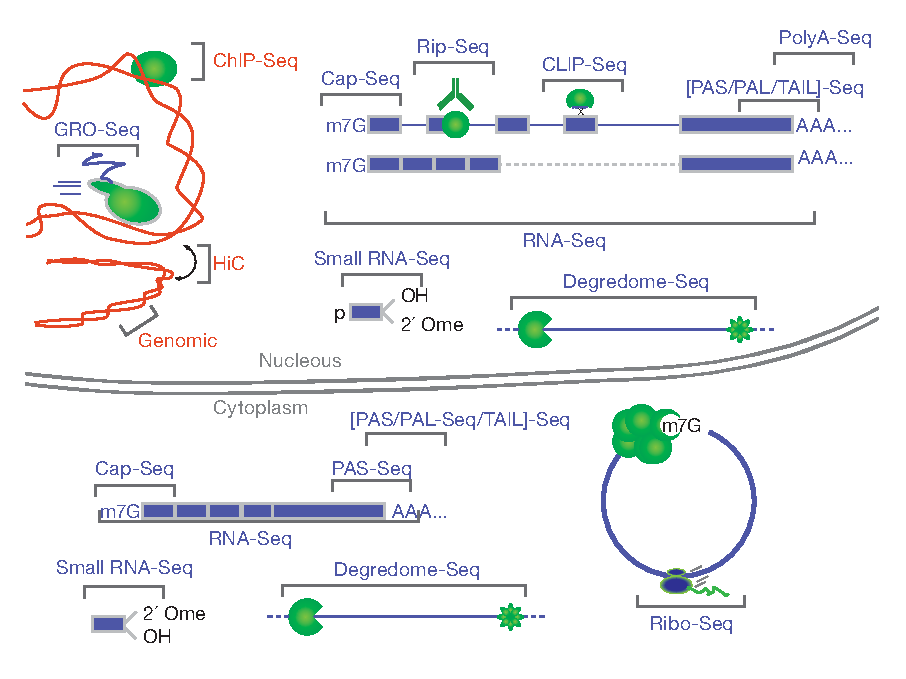
\includegraphics{Figures/Intro/RNA_Sequencing_methodologies.eps}
      \caption[Methods for High-throughput sequencing of RNA]
      {
      Methods for High-throughput sequencing of RNA\\[0.25cm]
      In the short years since the first report of RNA-Seq, many variations have been reported. The figure above provides an incomplete graphical illustration of some of these variations. A more complete list of *Seq applications is maintained on this \href{http://liorpachter.wordpress.com/seq/}{blog}.
      }
      \label{Intro:fig:htsMethods}
      \end{figure}

    RNA processing begins the moment the nascent RNA is exposed from the polymerase exit channel. Numerous methodologies enrich RNA-Seq libraries for particular types of RNA. For example, measurement of nascent transcripts can be performed via GRO-Seq \citep{Core2008a}, and the extremely complicated process of RNA turnover (referring to the rates at which RNAs both are produced and degraded) has been examined \citep{Ghosh2010a, Tani2012}. RNA::Protein interactions can be measured with or without cross-linking the protein to the RNA, via CLIP or RIP, respectively \citep{Ule2005,Licatalosi2006,Singh2013}. Once an RNA has been fully transcribed, known processing steps such as 5\textprime~7meG (CAP) formation and poly(A+) tail formation can be measured using any of the Cap-Seq/CAGE methodologies \citep{Shiraki2003a}, or PAS/TAIL/PAL \citep{Shepard2011, Chang2014b, Subtelny2014}. With appropriate size-selection steps, small RNAs \citep{Ghildiyal2008} can also be captured into a sequencing library. Finally, traditional RNA-Seq, can effectively capture fragments of all of the above mentioned libraries, even though it is mainly associated with measurement of traditional mRNAs.

    RNA-Seq (and all its flavors) are traditionally associated with quantification of RNA obtained from \textit{many} tissue culture cells or bulk pieces of tissue. Recently, efforts to measure RNA expression occurring in individual cells has gained attention \citep{Shapiro2013b}. Perhaps the most interesting concept when thinking about measurement of gene expression in a single cell is the ``biological uncertainty principle'', wherein it is possible to either know, or change --- but not both---~the RNA composition of a single cell. The name borrows from Heisenberg's uncertainty principle \citep{Kennard1927} and is often confused with the more appropriate ``Observer effect'' \citep{Riley2013}. Leaving that issue aside, measuring the unique transcriptome of a given cell is surly an exciting and informative endeavor \citep{Marinov2013, Shalek2013b,Wills2013}. Compared to DNA, the diversity of RNA synthesis within living cells is potentially much more complicated \citep{Shendure2012}, and the ability to accurately measure RNA dynamics should allow us to make much more informative observations concerning biology then is currently possible \citep{Djebali2012}.

\section{Nucleic Acid Splicing}
  \label{Intro:sec:Nucleic Acid Splicing}

  1977 brought the discovery of ``split genes'' \citep{Berget1977a,Chow1977}. Almost immediately after, it was reasoned that split genes could be arranged in different combinations, greatly increasing the coding potential of a genome \citep{Gilbert1978a}. The process of rearranging genes, now known as alternative splicing (AS), has proven to be an integral phase of gene expression in most eukaryotes. 

  \subsection{Alternative Splicing}\label{Intro:subsec:Alternative Splicing}

    The number of genes estimated to be alternatively spliced has grown considerably. In 1993, Phillip Sharp, Co-Nobel-prize winner for the discovery of splicing, stated that: ``Approximately, one of every twenty genes is expressed by alternative pathways of RNA splicing in different cell types or growth states'' \cite{Sharp2014}. Not long after the assembly of the first human genome, a number of groups combed through Expressed Sequence Tag (EST) databases to increase that estimate to 35\%-59\% \citep{Modrek2002}. Soon after, analysis using specially designed microarrays resulted in an increased estimate of 74\% \citep{Johnson2003}. However, in late 2008, three groups used RNA-Seq to demonstrate that between 86\% and 95\% of human multi-exon genes are subject to AS \citep{Pan2008, Wang2008, Sultan2008}. Not only did they demonstrate that almost all genes are alternatively spliced, they also showed that AS often occurs in a tissue- and cell type-specific manner. In combination with regulation of transcription itself, the study of AS is critical to our understanding of the connections between the comparably static genomic DNA sequence and the highly flexible and adaptive abilities of organisms.

    A pair of papers recently published in Science best illustrate the amazing complexity AS can generate between, and perhaps more importantly \textit{within}, organisms \citep{Barbosa-Morais2012,Merkin2012}. Analysis of RNA obtained from a diverse array of organisms and tissues by RNA-Seq has revealed that splicing patterns are shared more closely between organs of different species than between different organs of the same species. It seems that Alternative splicing contributes greatly to utilization of a common genome to role required by physiologically-specialized organs. 

    \begin{figure} % # of Genes and % Alternatively Spliced
      \centering 
      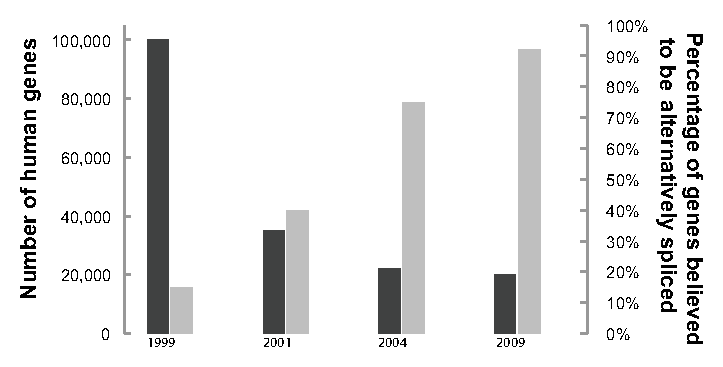
\includegraphics{Figures/Intro/numberHumanGenesAndNumberSpliced}
      \caption[Estimates of number of human genes, and percentage alternatively spliced over time]
      {
      Dark Grey - Estimates of number of human genes; Light Grey - Estimates of what percent of genes undergo some form of alternative splicing.
      }
      \label{Intro:fig:numGenesAndNumSpliced}
      \end{figure}


  \subsection{Deciphering a splicing code}\label{Intro:subsec:Splicing Code}

    A gene is alternatively spliced when, as a result of transcription and processing, there are at least two unique transcripts produced from one genomic sequence. Beyond isoform counting by RNA-Seq, a major area of effort is decoding sequence regulatory elements (SREs) contained in pre-mRNA that define AS site selection \citep{Wang2008}. In contrast to core splicing signals, there exists limited knowledge of the SREs that serve to increase and decrease, the strength of a particular splice site. Regulatory elements are always surrounded by a sea of other potential sites. Through a variety of mechanisms, SREs serve as cis-acting sequences and binding sites for trans-acting factors. Some of the best-studied SREs include Exon Splicing Enhancers and Silencers (ESEs and ESSs). Members of the Serine-Arginine (SR) protein family typically bind to ESEs located in an exon, promoting exon definition and thereby increasing the probability that the exon will be included in the final transcript \citep{Graveley2000,Long2009}. Meanwhile, ESS recognition  squelches inclusion through binding trans-acting heterogeneous ribonucleoprotein particles (hnRNPs) \citep{Martinez-Contreras2007}. Therefore, trans-acting factor SRE binding can either promote or inhibit splicing machinery::pre-mRNA interactions. The current working hypothesis is that a finely tuned combination of these binding events determines the final exonic content of each isoform \citep{House2008}.

    Sequence motifs that compose the AS code have been teased out \citep{Ladd2002, Barash2010}. Additionally, assignment of binding motifs to tissue-specific trans-acting factors has also progressed \citep{Jin2003,Ule2005,Licatalosi2008}. Many of these binding motifs were identified using combined computational and biochemical approaches. Computational approaches usually involve searching for a comparative enrichment of sequences near splice sites. Biochemical approaches include gel shift, SELEX, and cross-linking. Many of these approaches are performed in vitro and disregard the importance of cellular context on binding affinities. However, with increasing accessibility of HTS, many groups are extracting physiologically relevant, high-resolution data from traditional biochemical techniques \citep{Ingolia2009, Ingolia2011}. Deep-sequencing approaches are also being applied to questions involving mechanisms of AS. In addition to the RNA-Seq experiments, High-Throughput Sequencing [following] Cross-Linking Immunoprecipitation (HTS-CLIP) has confirmed SRE motif data predicted from computational and microarray experiments \citep{Licatalosi2008,Hafner2010}. Using HTS-CLIP, researchers can now enrich their samples for sequences that bind trans-acting factors of interest. 

  \subsection{The Isoform Problem}\label{Intro:sec:Isoform Problem}

    AS research now relies on large-scale (aka: \textit{global, genome-wide, high-throughput}) techniques. Two of the most widely-applied technologies employed for large-scale analysis of gene expression are microarrays and ``2nd generation'' HTS. Unfortunately, both of these techniques have fundamental limitations, with the major issues being probe specificity for the former and read length for the latter.

    \begin{figure} % Seqlengths and Connectivity
      \centering 
      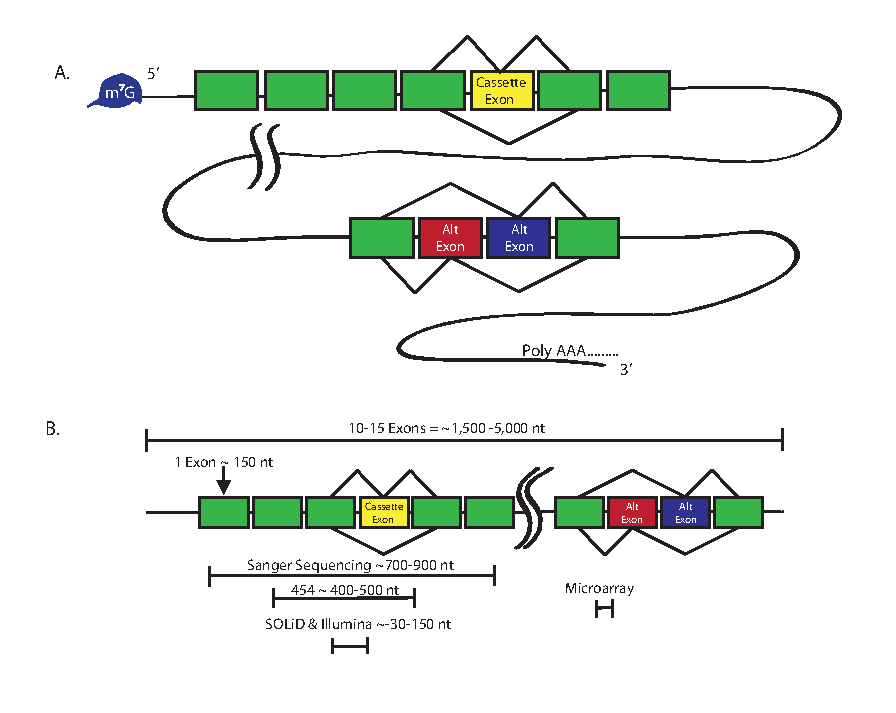
\includegraphics{Figures/Intro/SeqLengths_and_Connectivity.eps}
      \caption[HTS read lengths are not sufficient to maintain AS connectivity]
      {
        HTS read lengths are not sufficient to maintain AS connectivity\\[0.25cm]
        A) Long RNAs may have multiple sites of AS, separated by 1000's of nt; B) Most mRNAs have\textasciitilde10 exons of\textasciitilde150 nt each. Some have many more (and longer) exons. Read lengths of current sequencing technologies do not maintain connectivity between distant sites.
        }
      \label{Intro:fig:NoConnectivityInHTSMethods}
      \end{figure}

    Microarrays rely on hybridization of a target sequence to a known probe averaging 25-- 100 nt in length \citep{Southern2001}. Therefore, microarrays  only report the presence of short sequences in the target sample and do not provide linkage information between the sequences. A hypothetical scenario can be used to describe this issue. The goal of this example is to investigate a transcript known to display two different regions of AS (see Figure \ref{Intro:fig:NoConnectivityInHTSMethods}). Probes targeting these two regions demonstrate an increase in signal for both AS events. Unfortunately, it is not known if we observe an increase in unique transcripts, each containing only one region of AS, or an increase in production of a single transcript containing both regions \citep{Calarco2007}. This binary analysis is the heart of the ``connectivity problem.'' Microarrays have proven extremely informative and will likely continue to do so in more targeted applications. However, this issue, combined with concerns of cross-hybridization, reproducibility, and a comparably small dynamic range, has hastened the displacement of microarray by RNA-Seq as the preferred method for comprehensive analysis of gene expression \citep{Shendure2008}.

    2nd generation HTS methodology is the \textit{de facto} method for comprehensive transcriptome analysis. HTS allows for \textit{de novo} identification of isoforms. RNA-Seq operates over a larger dynamic range and in a quantitative manner \citep{Mortazavi2008}. Additionally, techniques exist to enrich samples for low-abundance isoforms, making the complete cataloging of AS events a possibility \citep{Djebali2008, Salehi-Ashtiani2008}. Unfortunately, the current read-length abilities (see Figure \ref{Intro:fig:NoConnectivityInHTSMethods}) of all sequencing platforms do not solve the connectivity problem. Excluding single-molecule read lengths of sufficient length \citep{Shendure2004}, other approaches proposed to solve the connectivity problem include traditional cloning and sequencing or hybridization of query oligos to single-molecule transcripts \citep{Zhu2003, Calarco2007, Emerick2007}. While these approaches can determine exon sequence connectivity, they scale poorly and are not feasible for large-scale applications.

    AS is an essential regulatory mechanism involved in the control of human gene expression. Its combinatorial nature could potentially answer many basic questions concerning gene expression, such as a physical explanation of what separates us from our closest evolutionary ancestor, the chimpanzee \citep{Calarco2007a}. Additionally, the influence of AS on disease and cancer is slowly coming to light \citep{Tazi2009}. Unfortunately, because of the limitations of methods currently used for the large-scale analysis of isoform expression, we fail to obtain the complete picture of AS. One specific missing element of that picture is the prevalence of coordination between different regions of AS separated by large spans of sequence. An efficient, large-scale, single-molecule technique that maintains isoform sequence connectivity is required to complete the complicated picture of AS.

    Identification of proximally-acting SREs is progressing at a rapid pace. New and traditional biochemical methods, coupled with HTS, will undoubtedly fuel this progress. Unfortunately, a critical component of AS regulation currently neglected by the field is that of SREs acting across a considerable distance (>800 nt). One observation that may lead to the identification of long-range SREs is intramolecular coordination between distal splicing decisions. In Figure \ref{Intro:fig:NoConnectivityInHTSMethods} a model transcript that may exhibit coordinated distal regions of AS. In this model, the 5\textprime~region of AS contains a cassette exon, which may or may not be included. This region is separated from the 3\textprime~region of AS by many thousands of nucleotides. Does the decision to include the cassette exon have an effect on which of the mutually exclusive exons is included? This type of AS regulation may represent a general and pervasive phenomenon.

  \subsection{Coordination in splicing}\label{Intro:subsec:Coordination in splicing}

    The provocative ``Miller Spread'', showing spliceosomes associated with RNA transcripts, ignited the first thoughts that transcription and splicing are intricately linked \citep{Osheim1985}. Twelve years later, the observation that polymerase speed can affect downstream splicing decisions was reported \citep{Cramer1997}, spawning a new field of research into linked transcription and splicing. But how linked are these two processes? 

    How would linkage between transcription and splicing manifest? One of the clearest examples is mouse Fibronectin \fn{} (see Figure \ref{Intro:fig:mouseFn1}) \citep{Schwarzbauer1983, White2011a}. In this gene, inclusion of the alternatively spliced Extra Domain A (aka ``EDI'' or ``EDA'') region promotes splicing from one of three alternative 3\textprime~Splice Sites (3\textprime~SS) in the type III homology connecting segment (IIICS) region, resulting in more frequent production of shorter transcripts \citep{Fededa2005}. This effect occurs over six constitutively expressed exons and 800 nt of sequence (5400 nt if introns are considered). \citep{Fededa2005} also analyzed EST databases, concluding that approximately 25\% of human genes contain multiple regions of AS. How many of these regions could show a coordinated effect, similar to that observed in \fn{}? Providing some insight into this question, \citep{Fagnani2007} used microarrays designed to report on inclusion levels of cassette exons in mammalian central nervous system tissues \citep{Fagnani2007}. The results produced a set of 38 pairs of exons mapping to the same gene that showed a coordinated increase or decrease of inclusion levels. 

    \begin{figure} % Fibronectin Architecture Figure 
      \centering 
      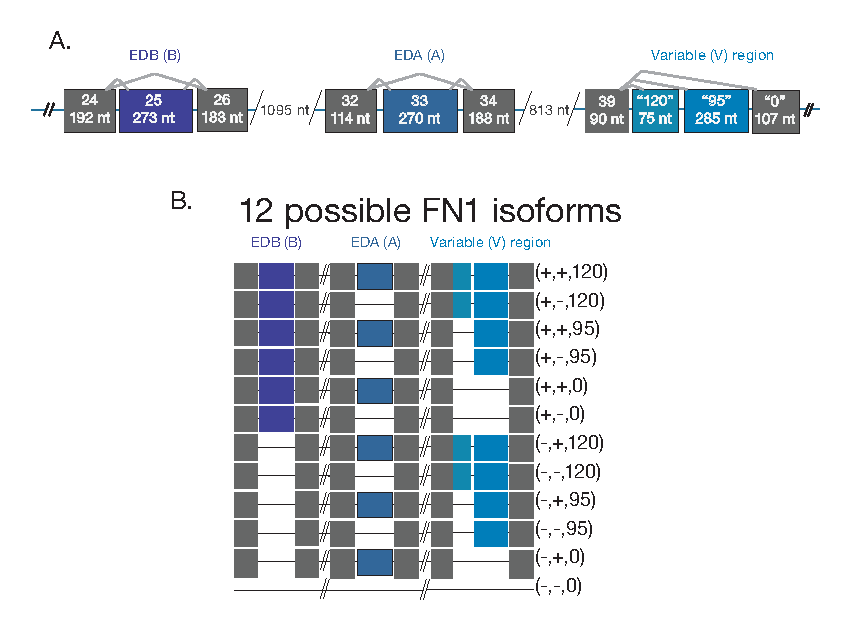
\includegraphics{Figures/Intro/Fibronectin.eps}
      \caption[Mouse \fn{} contains multiple sites of Alternative Splicing]
      {
        Mouse \fn{} contains multiple sites of Alternative Splicing\\[0.25cm]
        A) There are three highly-studied regions of AS in mouse \fn{}: The cassette exons EDB and EDA, and the Variable(V)-region exon, which displays multiple 3\textprime~splice sites.  Each of these sites is separated by multiple constitutive exons. B) Considering simplistic splicing of these three exons, there are 12 different isoforms of mouse \fn{}.
        }
      \label{Intro:fig:mouseFn1}
      \end{figure}

    Few studies have investigated coordinated splicing between adjacent exons present in mRNA. The vertebrate genes \textit{4.1B} and \textit{4.1R}, members of the protein 4.1 family encode cytoskeletal adaptor proteins. Both genes undergo splicing of upstream 5\textprime~first exons to distal 3\textprime~second exons, skipping a stronger proximal 3\textprime~second exon \citep{Parra2008, Parra2012}. This is accomplished through ``intrasplicing'' involving an intronic sequence element (``intraexon'') only present when transcription begins at the upstream 5\textprime~exon. This allows the exon to ligate to the weaker distal 3\textprime~second exon via an intermediate splicing event. Importantly, this type of splicing would be similar, but different from, recursive splicing seen in drosophila \citep{Burnette2005a}.

    Another example of the importance of Intronic Recognition Elements (ISE) on AS is that observed in equine \textit{$\beta$-casin}, where the authors propose a model involving an IRE bound to the exit channel of the elongating polymerase. IRE binding promotes inclusion of downstream cassette exons \citep{Lenasi2006}. Taking a more genome-wide approach \citet{Peng2008} examined human and mouse EST data looking for correlations between adjacent AS cassette exons. The authors note that positively correlated pairs of adjacent cassette exons typically resemble constitutive exons in splice strength, whereas negatively, or weakly correlated pairs are likely to be newly emerging exons, whose strength of splicing has not evolved enough to be constitutively included.

    The last, most current, and thorough study of intra-gene splicing coordination involves the \worms{} gene \slo{} \citep{Glauser2011, Johnson2011}. \slo{} is the \worms{} orthologue of the human BK channel gene \kcnma{}, also known to undergo extensive alternative splicing \citep{Nilsen2010} via 13 cassette exons, potentially coding for over 1,000 different isoforms. \kcnma{} is highly developmentally, spatially, and tissue regulated. It is involved in a diverse range of cellular processes, including hearing, circadian rhythms, urinary function, and vasoregulation \citep{Fodor2009a}. While the gene is highly conserved, as organism complexity grows, so does the apparent transcriptional diversity of this gene. In worms, \slo{} can produce up to 12 different isoforms. \citet{Glauser2011} used QPCR to demonstrate individual, AS region inclusion frequencies do not correspond to complete isoform frequencies, when measured via TaqMan. They go on to describe a interdependent-splicing model that best fits the data, and support interdependence via mutations at one sight altering splicing at both upstream and downstream sites of AS, separated by at least one other splicing event. After measuring the biophysical properties of the isoforms \citep{Johnson2011}, they conclude that coordinated AS is critical for proper BK channel function in vivo. It is interesting to note that this study also identified an IRE that displayed some type of coordinated, or co-regulated effect on AS.

    Indeed the ``Miller Spread'' was an early glimpse into another aspect of Nature's complexity. Over just the past \textasciitilde5 years, layers of functional coupling between transcription and splicing have been observed \citep{Merkhofer2014}. For example, specific chromatin marks seem to not only demarcate transcriptionally active regions of chromatin for silent ones, but also AS exons from constitutively chosen ones \citep{Kolasinska-Zwierz2009} and first exons appear to be epigenetically marked to aid in transcriptional identification \citep{Bieberstein2012}. Tied to the recurring theme of this thesis, increasing resolution of genome-wide data should reveal more and more ties between these cellular processes \citep{Schwartz2010,Luco2011a,Brown2012}.

  \subsection{Many isoforms per gene}\label{Intro:subsec:IsoformsPerGene}

    Just as it is tempting to uncouple what are evolutionarily intertwined processes such as transcription and splicing, it is easy to think of AS as a binary process. Isoform A or B is produced based upon picking either exon A or B. What quickly becomes evident, and is far too real for researchers building transcriptome assembly algorithms, is that the combinatorial nature of AS makes it both a power means of generating isoform diversity \textit{and} a difficult problem to study \citep{Trapnell2012a}.

    \begin{figure} % AS Events per type barchart
      \centering 
      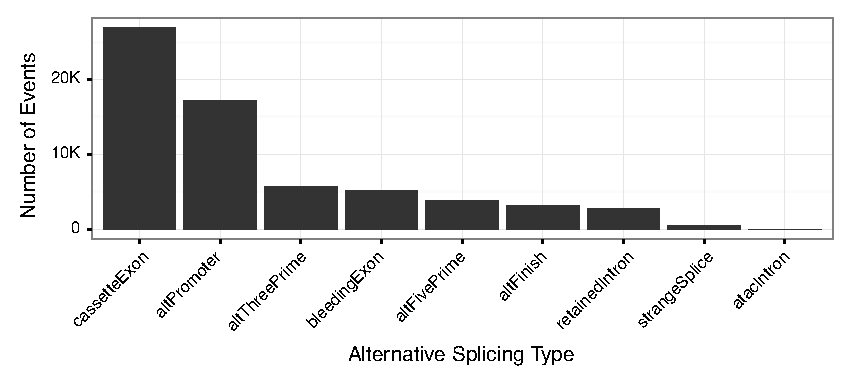
\includegraphics{Figures/Intro/ASEventTypesPlot.eps}
      \caption[Number of hg19 Alternative Event types per gene]
      {
        Number of hg19 Alternative Event types per gene\\[0.25cm]
        Alternative Event types per gene. Accessed from RefSeq on 2014-03-24.
        }
      \label{Intro:fig:asEventsBarChart}
      \end{figure}

    One of the most recent attempts to investigate the breath of combinations produced by AS is the ENCODE project \citep{Birney2007,Dunham2012}. The transcriptional annotation arm of the ENCODE project \citep{Djebali2012,Derrien2012} used the data from extremely in depth analysis of 15 human cancerous cell lines, and found that each gene produces \textasciitilde10 isoforms per gene, with a broad distribution in terms of isoforms expressed per sample. 

    The ENCODE project demonstrated added to the building evidence that most human genes undergo AS in many more ways than previously appreciated \citep{Wang2008,Pan2008}. Most genes could be considered as undergoing ``complex'' AS, with numerous forms of AS (see Figure \ref{Intro:fig:asEventsBarChart}). Despite the prevalence of complex alternative spliced genes, few genes are routinely used as examples to illustrate numerical possibilities and biological significance. For example the human immune system relies heavily on AS for plastic antigen recognition and response \citep{Lynch2004}. Modulation of extracellular signaling proteins such as \textit{CD44} and cellular adhesion protein \textit{CD45} have been well-studied \citep{Zikherman2008,Ponta2003}. Alternative splicing in humans, however, does not seem to produce the number of unique possible combinations as AS of genes in simpler organisms, such as \flies{} (see Figures \ref{Intro:fig:txPerFlyGene} and Table \ref{Intro:fig:txPerFlyGene}). Perhaps this reduced AS \textit{per gene} is due to specialization of genes, with different genes working in combination, as oppose to utilizing unique isoforms from a single gene \citep{Park2007}. For example, the fruit fly gene muscle myosin heavy chain (\textit{Mhc}) can produce up to 480 different isoforms through AS of 17 different cassette exons \citep{Bernstein1983a}. Section \ref{Intro:subsec:Dscam} will discuss an even more appropriate comparison between the human and fly extracellular binding protein DSCAM.

    \begin{figure} % Number of transcripts per gene
      \centering 
      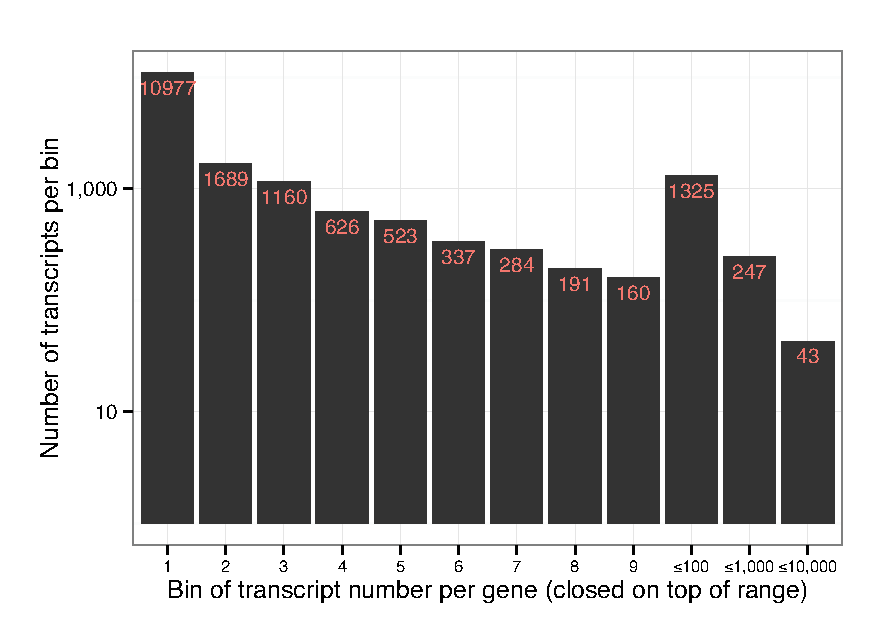
\includegraphics{Figures/Intro/NumberOFTranscriptsPerFlyGene.eps}
      \caption[Number of transcripts per \flies{} gene]
      {
        Number of transcripts per \flies{} gene\\[0.25cm]
        Data from \citep{Brown2014}, Supplemental Table 3. Number of transcript per bin, with bin sizes ``closed'' on the upper part of range.
        }
      \label{Intro:fig:txPerFlyGene}
      \end{figure}

    \begin{table} % Fly genes with 1000's of Tx
      \caption{Fly genes with >2,000 assembled transcripts according to \citep{Brown2014}.}
      \label{Intro:tab:FlyGenesWithManyTx}
      \renewcommand{\arraystretch}{0.5}
\small
\begin{tabular}[c]{l|r|r|r}
	\hline
	\textbf{Gene Name} & \textbf{\# Introns} & \textbf{\# Transcripts} & \textbf{\# Proteins}\\
	\hline
	Mhc & 60 &  2040 & 511\\
	\hline
	slo & 49 &  2070 & 279\\
	\hline
	ps & 30 &  2099 &  27\\
	\hline
	rg & 45 &  2178 &  23\\
	\hline
	shot & 60 &  2478 & 886\\
	\hline
	scrib & 53 &  2555 & 259\\
	\hline
	heph & 75 &  2876 &  52\\
	\hline
	CG42748 & 26 &  2876 &  51\\
	\hline
	rdgA & 35 &  3003 &  89\\
	\hline
	Mbs & 39 &  3080 & 119\\
	\hline
	CaMKI & 41 &  3992 &   7\\
	\hline
	par-1 & 48 &  4410 & 142\\
	\hline
	GluClalpha & 27 &  4945 & 188\\
	\hline
	Sap47 & 24 &  5011 &  49\\
	\hline
	Patronin & 50 &  5615 & 590\\
	\hline
	CG17838 & 37 &  8333 & 147\\
	\hline
	unc-13 & 52 &  8391 & 279\\
	\hline
	A2bp1 & 29 &  9055 &  58\\
	\hline
	Imp & 33 &  9131 &  12\\
	\hline
	pan & 38 &  9432 &  72\\
	\hline
	Sh & 40 & 15995 &  66\\
	\hline
	gish & 48 & 18972 & 142\\
	\hline
  \end{tabular}
      \end{table}

  \subsection{\flies{} \dscam{}}\label{Intro:subsec:Dscam}

    Unquestionably, the gene most frequently used to demonstrate the combinatorial power of AS is \flies{} \dscam{}. The ``architecture'' of \dscam{} is rather unique, but as we see in Figure \ref{Intro:fig:txPerFlyGene} and Table \ref{Intro:fig:txPerFlyGene}, \flies{} contain numerous genes that generate tremendous isoform diversity from a single genetic locus \citep{Brown2014}. The basic structure of \dscam{} is shown in Figure \ref{Intro:fig:DscamArch}.

    Human \textit{Dscam} (Down Syndrome Cellular Adhesion Molecule), for which \dscam{} was named, was identified while looking for genes on chromosome 21, specifically band 21q22, where extra copies expressed in Down syndrome patients, a trisomy 21 disorder, may be causative for disease \citep{Yamakawa1998a}. \textit{Dscam} was named according to this association, and its membership in the immunoglobulin super family of proteins with extracellular adhesion functions. Human \textit{Dscam} does undergo some alternatively splicing and is broadly expressed in the developing nervous system. Yet, it does not contain the impressive number of cassette exons as \dscam{}.

    \begin{figure} % Dscam Architecture
      \centering 
      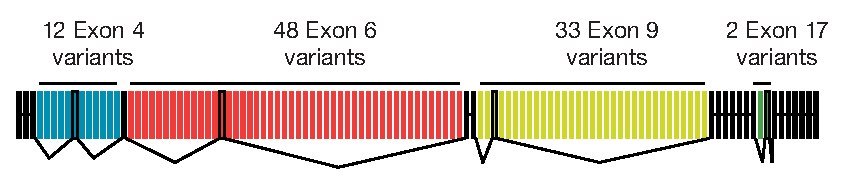
\includegraphics{Figures/Intro/DscamArch.eps}
      \caption[The architecture of the \flies{} gene \dscam{}]
      {
        The architecture of the \flies{} gene \dscam{}\\[0.25cm]
        \dscam{} has three \textit{clusters} or ``banks'' of alternative cassette exons that are splicing out in a mutually-exclusive manner. The first bank, ``Exon 4'', contains 12 different variants, of which one one is ever included into the mRNA. Similarly, banks 6 \& 9 each contain 48 and 33 different variants, respectively. These three banks code for extracellular IgG domains, while the final region of AS, exon 17, encodes two different trans-membrane domains, again of which only one is included in the final mRNA.
          }
        \label{Intro:fig:DscamArch}
        \end{figure}

    Complex AS of\dscam{} was first noticed by the Zipursky lab in 2000 \citep{Schmucker2000}. While looking for proteins associated with \textit{dock} and \textit{pak}, two proteins important for neuronal growth cone guidance, they biochemically co-purified DSCAM1. Sequencing of \dscam{} clones revealed that virtually clones contained different combinations of exons 4,6, and 9. In fact, these three exons are chosen from three clusters of mutually-exclusive cassette exons, containing 12, 48, and 33 different options each (see Figure \ref{Intro:fig:DscamArch}). The initial report kicked off an exciting period of research into \dscam{} structure and function. Determining the mechanism and functional significance of \dscam{} isoform diversity was a major goal of multiple labs.

    Before the highlights of \dscam{} research are reviewed, it is illustrative to discuss some basic \flies{} anatomy. There are 4 main regions where \dscam{} expression has been highly-studied. These four biologically important roles are shown in Figure \ref{Intro:fig:DscamAnatomy}.

    \begin{itemize} \itemsep0.5pt \parskip0pt \parsep0pt % Dscam expression regions
      \item Hemocyte cells of the immune system
      \item Larva Class IV da Neurons 
      \item Pupal Mushroom-body neurons in the developing brain
      \item Tetrad synapses of the eye
      \end{itemize}

    During larval development, \dscam{} is expressed in the da neurons of the larval body wall. Da neurons create a uniform sensory field, allowing larva to respond to mechanical stimulus. Morphologically, da neurons resemble an oak tree growing in a sunny field, allowing the larvae to sense as much as possible. In order to maximize coverage of the field, every Cell::Cell interaction (i.e. every synapse) must be a productive one. Molecularly, this is accomplished via an extracellular handshake between two copies of DSCAM1. If this handshake feels too familiar, a stable, lasting, and \textit{productive} synapse is actively discouraged until a new and different handshake is felt \citep{Wojtowicz2004}. The use of DSCAM1 to discern self from non-self determination is not unique to da neurons. It is also essential for an equally critical, and arguably more complex, nervous systems including the eye and brain. In the developing brain, \dscam{} is expressed in both axonal projections of neurons extend from Kenyon cell bodies and bifurcate into the two different mushroom body lobs \citep{Zhan2004}. Finally, the involvement of \dscam{} in the innate immune system of insects has been demonstrated \citep{Watson2005,Dong2006}.

    \begin{figure} % Dscam Anatomy
      \centering 
      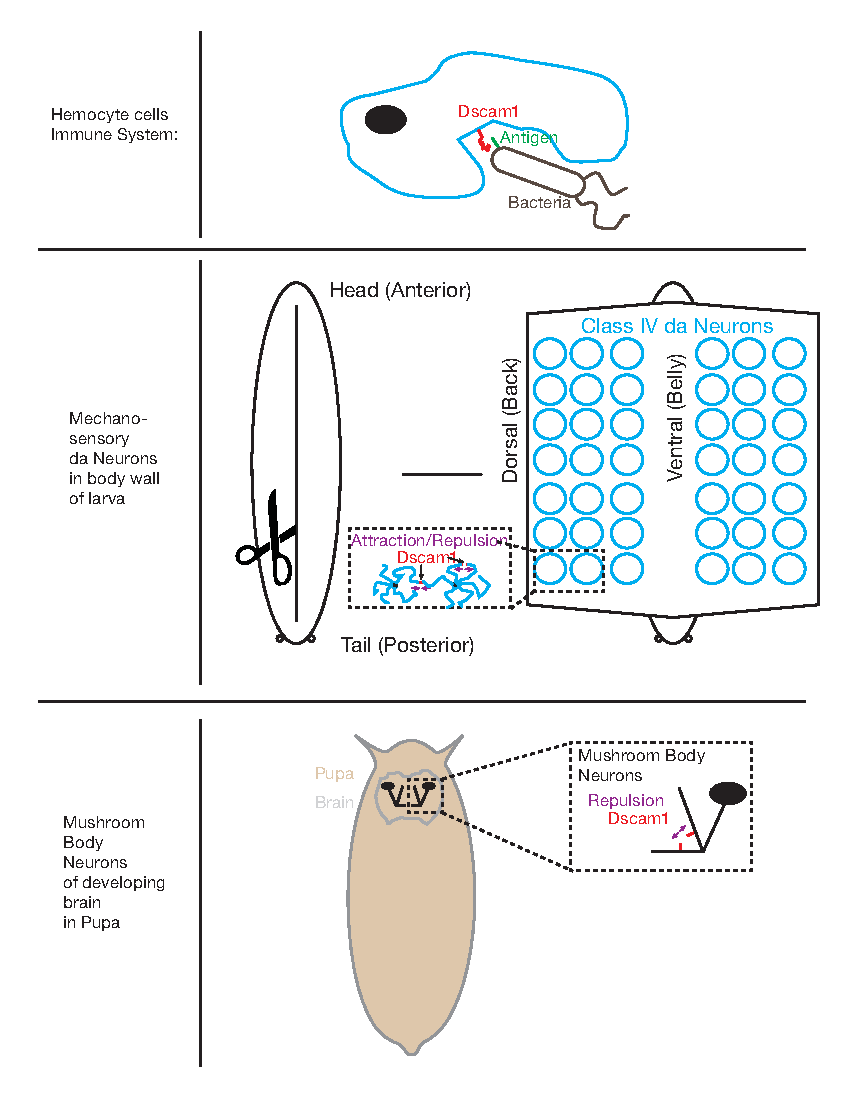
\includegraphics{Figures/Intro/DscamAnatomy.eps}
      \caption[Important \dscam{} expression during \flies{} life cycle]
      {
        Important \dscam{} expression during \flies{} cycle\\[0.25cm]
        \dscam{} has been high-studied in four different regions/cell types. 1) Hemocytes of the immune system, where DSCAM1 is involved in antigen recognition; 2) In Class IV da neurons, which sense mechanical stimulation of the larval body wall; 3) In mushroom body neurons of the pupal developing brain; and 4) (not shown) in Tetrad neurons of the eyes.
        }
      \label{Intro:fig:DscamAnatomy}
      \end{figure}

    With the functionally significance of \dscam{} expression clear, it is important to review research into the mechanisms of generating tremendous isoform diversity. Soon after the initial \dscam{} report \citet{Celotto2001} investigated the genes developmental regulation. They focused on the 12 variants of cluster 4 and observed regulation of exon 4.2. Embryonic transcripts show little inclusion of this exon, while adult transcripts show frequent inclusion. Exon 4.8 demonstrates the opposite behavior. Similar regulation of cluster 4 exons was also observed in a closely related species, \textit{Drosophila yakuba}.

    In 2004, \citet{Neves2004} used a specially designed microarray to robustly characterize \dscam{} molecular diversity. They observed, at some rate, inclusion of virtually all alternative exons from clusters 4, 6, and 9. Additionally, they examined \dscam{} transcripts obtained from colonies grown from single cells and reported that multiple \dscam{} transcripts were expressed per cell, estimating between 7-- 50 different combinations per cell, depending on the cell type. As discussed above, the use of microarrays to perform this analysis precluded observing any potential coordination between variant exons.

    Quickly after \citet{Neves2004} published their results, the Zipursky lab also published a microarray study of \dscam{} isoforms \citep{Zhan2004}. They focused their analysis on neurons of the developing Mushroom body (see Figure \ref{Intro:fig:DscamAnatomy}). Not only did they also show that most \dscam{} combinations are likely produced at some level, but that diversity of isoforms is required for bifurcation of neurons into different lobes of the developing mushroom body. These results highlighted a critical function for DSCAM-- mediating extracellular interactions via homophillic binding.

    How is mutually-exclusive exon usage among 48 different options possible? \citet{Graveley2005b} observed a single ``Docking site'' within the intronic sequence just 5\textprime~to exon 6.1. This docking site was conserved among 15 insect species examined, from closely-related \textit{Drosophila simulans} to a distantly-related \textit{Tribolium castaneum} (Red flour beetle). Astonishingly, the docking site was complementary to ``Selector sites'' within intronic regions just 5\textprime~of each of the 48 variant exons. A model is proposed where Docking::Selector interaction is required to choose which variant exons is included, while a splicing regulator protein, likely an hnRNP due to the repressive nature of the interaction, binds to unused selector sites contained in the pre-mRNA \citep{Graveley2000}. Additional mechanisms have been reported for other clusters, including the \textit{iStem} \citep{Kreahling2005} in cluster 4, and the hnRNP protein hrp36 \citep{Olson2007}.

    \citep{Neves2004} examined \dscam{} expression in hemocyte cells, and their results clearly show reduced variability in cluster 9 inclusion. Virtually all of the signal obtained from hemocyte cells for cluster 9 was seen in variants 9.[6,9,13,30,and 31]. \citep{Watson2005} also examined \dscam{} expression in hemocyte cells, comparing it to that of neuronal cells. They propose that secreted forms of \dscam{} are essential for a robust innate immune system in insects. These studies highlight how nature has applied one gene that produced extreme molecular diversity to multiple problems involving determining self from non-self \citep{Shi2012a, Hattori2008}. \dscam{} use in these two very different biologically roles has been summarized previously \citep{Hemani2012}.

    In 2007 the Zipersky lab published \citep{Hattori2007} the first in a series of quality genetic reports describing the function and diversity of \dscam{}. Using homologous recombination, \citet{Hattori2007} showed that \dscam{} diversity is required for proper neural wiring but that individual neuronal-isoform identity is not important. Two years later, \citet{Hattori2009} observed that flies capable of expressing at least 4,752 different \dscam{} isoforms were indistinguishable from wild-type controls. This series was recently advanced with another tour-de-force of genetic manipulation. \citet{Miura2013b} used a collection of \dscam{} mutants allowing for visualization via GFP of specific cluster 4.X variant expression in real time. They concluded that a single neuron expresses multiple \dscam{} isoforms over time, and \dscam{} is expressed via ``stochastic and probabilistic'' mechanisms.

    Research into \flies{} \dscam{} has provided major advancements to our understanding of multiple aspects of transcription, including: 1) Exon definition; 2) Alternative Splicing of cassette exons; 3) Neuronal and cellular recognition; and finally 4) Allowing comparisons between how points 1--3 are accomplished in ``simple'' model systems and humans. See sections \ref{SeqZipPaper:sec:Results}, \ref{Disc:sec:Dscam} for more information concerning \dscam{}.

\section{Nucleic Acid Ligation}
  \label{Intro:sec:Nucleic Acid Ligation}

  Biomedical research is advanced by countless technologies. Section \ref{Intro:sec:Nucleic Acid Sequencing} discusses implications of cheap sequencing DNA and RNA sequencing. This section discusses how the ability to \textit{join} pieces nucleic acid has also advanced our understanding of biology. A particular focus is placed on an enzyme with relevance to Chapters \ref{SeqZipPaper} and \ref{SeqZipMethod}--- T4 RNA Ligase 2.

  \subsection{RNA Sequence investigation by ligation}
    \label{Intro:subsec:Ligation}

    In the late 1960's and early 1970's, the Lehman and Richardson labs characterized two workhorse-enzymes of modern molecular biology. Robert Lehman and colleagues, working at Standford Medical School, first described the activity of \textit{polynucleotide-joining enzyme} from \textit{Escherichia coli} (now known as \textit{E. Coli} DNA Ligase) \citep{Olivera1967b}. Work on this enzyme paralleled that from the Richardson lab at Harvard Medical School, where they focused on \textit{polynucleotide ligase} from \textit{Escherichia coli} infected with T4 bacteriophage (now known as T4 DNA ligase) \citep{Weiss1967a}. It became clear that while these two enzyme's shared a common mechanism---later elucidated by \citep{Modrich1973a}---they had important differences. First, T4 DNA ligase required ATP as a cofactor, which \textit{E. Coli} DNA Ligase did not (it was later discovered that DNA ligase required NAD as a cofactor). Second, only T4 DNA ligase could catalyze ligation of blunt-ended DNA \citep{Tabor1987a}.

    \begin{figure}% Ligation Mechanism
      \centering 
      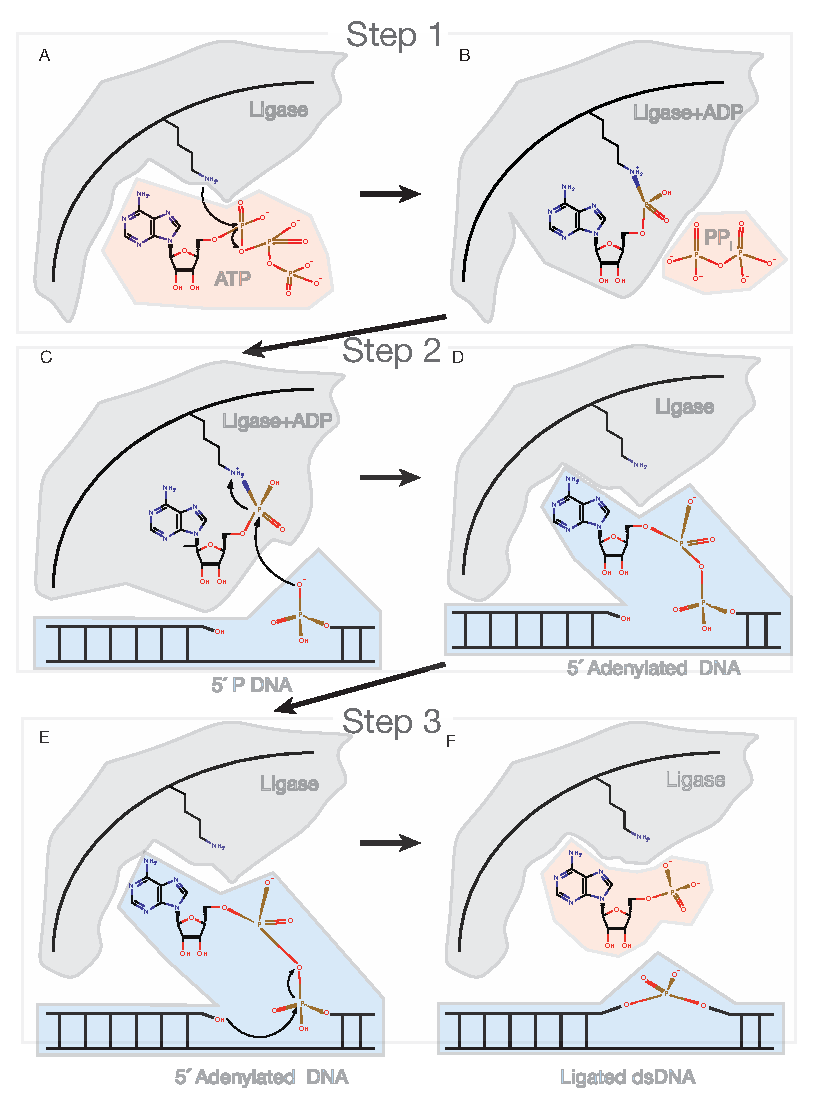
\includegraphics{Figures/Intro/LigationMechanism.eps}
      \caption[Mechanism of Rnl2 ATP-dependent ligation]
      {
        Mechanism of ATP-dependent ligation\\[0.25cm]
        Adapted from \citep{Nandakumar2006} and specifically for that of T4 RNA ligase 2.
        }
      \label{Intro:fig:Ligation Mechanism}
      \end{figure}

    The general mechanism of ligation, shown in Figure \ref{Intro:fig:Ligation Mechanism}, involves three steps: Step 1 (A) the $\epsilon$-amino group from the active site lysine performs a nucleophilic attack on the $\alpha$-phosphate of ATP in solution. B) The ligase is now charged with AMP and inorganic phosphate (PPi) is freed into solution. C) Step 2: Nucleophilic attack by the 5\textprime~DNA phosphate on the 3\textprime~side of the nick to the AMP:ligase phosphate. D) Adenylated DNA is now competent for DNA ligation. E) Step 3: the 3\textprime~OH on the 5\textprime~side of the nick performs a nucleophilic attack on the 5\textprime~PO$_{4}$ across the DNA nick, liberating AMP into solution. F) Sealed nick resulting in: Ligase; AMP; and intact dsDNA.

    In addition to elucidating the general mechanism of ligation, it was also discovered that T4 DNA ligase lacks a preference for terminal polynucleotide structures. The Khorana and Richardson labs both reported the activity of this enzyme on combinations of RNA and DNA duplexes \citep{Fareed1971, Kleppe1970b}. Both of these papers describe an activity on T4 DNA ligase, RNA-templated DNA to DNA ligation, that is of particular relevance to this thesis work. Unlike T4 DNA ligase, \textit{E. Coli} DNA Ligase, will not join DNA strands on an RNA template \citep{Bullard2006}. Soon after demonstrating these activities in vitro, the Khorana lab reported detection of organism-generated DNA \citep{Besmer1972b}, setting up an orthogonal field (respective to PCR) of nucleic acid sequence characterization \citep{Conze2009c}.

    An enzyme that can catalyze an RNA-templated DNA:DNA ligation is a very useful molecular biology tool for two main reasons. First, using RNA as a ligation guide means no modification is made to the template molecule. This contrasts cDNA analysis, where the RNA has been enzymatically converted by reverse transcription, potentially losing valuable RNA-coded information, such as modified bases. Second, synthesis of the DNA probes used in ligation is inherently easier and cheaper compared to synthesis of RNA probes. In addition to being cheaper, synthesis of DNA probes has become high-throughput since the adoption of microarrays as a standard gene expression measurement tool \citep{Schena1995a}. A pair of papers from the Landegren lab first reported the utility of RNA-templated DNA:DNA ligation for analysis of RNA transcripts \citep{Nilsson2000,Nilsson2001}. The Fu lab applied this approach in a multiplex experimental design in collaboration with Illumina \citep{Li2012c,Yeakley2002}, while Mats Nilsson and Ulf Landegren developed a single molecule application \citep{Conze2010}. It is important to note that \textit{all} of these studies used T4 DNA ligase. Clearly, there is interest and utility in analyzing RNA in both high-throughput and multiplex experimental designs, using cheap DNA probes, and without cDNA conversion.

    For more than 40 years after its first description, T4 DNA ligase was the only choice for RNA-templated DNA:DNA ligation. However, a recent publication from New England Biolabs (NEB) describes this activity by another well-studied ligase, Chlorella Virus PBCV-1 DNA ligase (herein Chlorella DNA ligase) \citep{Lohman2013c}. Chlorella DNA ligase is a long-studied enzyme and had been reported to \textit{not} display RNA-templated DNA:DNA ligation activity \citep{Ho1997b,Sriskanda1998c}. However, at high enough concentrations and under special buffer conditions (specifically a critical concentration of ATP), Lohman et al have shown that Chlorella DNA ligase will join two DNA strands hybridized to an RNA template \citep{Lohman2013c}. They further demonstrated that it performs no worse in this activity than traditional T4 DNA ligase \citep{Nilsson2001,Yeakley2002}.

    Building on the list of available enzymes that join hybrid polymer substrates Chapter \ref{SeqZipPaper} presents data supporting RNA-templated DNA:DNA ligation activity for another enzyme, T4 RNA Ligase 2.

  \subsection{T4 RNA Ligase 2 (Rnl2)}
    \label{Intro:subsec:Rnl2}

    Proteins of the T4 and T7 bacteriophages have been a boon for molecular biology. Without enzymes like polynucleotide kinase \citep{Richardson1965a}, T7 RNA polymerase \citep{Summers1970b}, and T4 DNA ligase \citep{Weiss1967a}, many essential manipulations of nucleic acids would have been impossible for decades. Obviously, these enzymes also have essential phage functions. T7 RNA polymerase is responsible for late stage replication of T7 phage transcripts, while T4 PNK works in concert with T4 DNA and RNA ligases to repair cleaved  nucleic acids resulting from bacterial pathogens defense systems \citep{Wang2002b}. Specifically, T4 RNA ligase 1 (herein ``Rnl1'', also known as \textit{gene 63} maintains phage replication by repairing tRNAs cleaved by an anticodon nuclease produces from the \textit{prr} locus \citep{Amitsur1987d}.

    Given the utility and importance of these enzymes, novel enzyme discovery is a fruitful area of research. The Shuman lab has a distinguished record of discovering and characterizing numerous such enzymes, including many involved in nucleic acid synthesis, modification, and repair. Through a blast search looking for novel ligases with sequences related to \textit{Trypanosoma brucei} RNA-editing ligases TbMP52 and TbMP48 \citep{Ho2002b}, they identified motifs in correct arrangement, spacing, and number indicative of an RNA ligase. The gene, identified as \textit{gp24.1}, has quickly become an essential tool in the era of modern genomics.

    Initial biochemical purification and characterization of \textit{gp24.1} \citep{Ho2002b} revealed that it indeed codes for an RNA ligase, which was renamed T4 RNA ligase 2 (herein ``Rnl2''). Rnl2 is a 374 amino acid monomeric protein composed of 2 distinct domains initially purified as a 42-kDA His-tagged recombinant protein. The N-terminal domain (1--243) is responsible for steps (1) and (3) of the general ligation mechanisms (see Figure \ref{Intro:fig:Ligation Mechanism}), while the C-terminal domain (244--329) is responsible for adenylation of the 5\textprime~PO$_{4}$ on the 5\textprime~residue at the 3\textprime~side of the nick, as shown in step (2). Additionally, Rnl2 is routinely purified as a pre-adenylated and immediately poised for its first ligation. In contrast to the N-terminal domain, which is composed of motifs typical to main ligases, the C-terminal domain is significantly  different from all other DNA ligases and has no structural homologue. While the biological function of Rnl1 is known, the biological function of Rnl2 remains a mystery, more than 12 years after its discovery \citep{Chauleau2013b}. However, there is some speculation that the flurry of research into bacterial CRISPR phage defense may reveal a role for Rnl2 \citep{Barrangou2007c,Chauleau2013b}.

    \begin{figure} % Rnl2 structure
      \centering 
      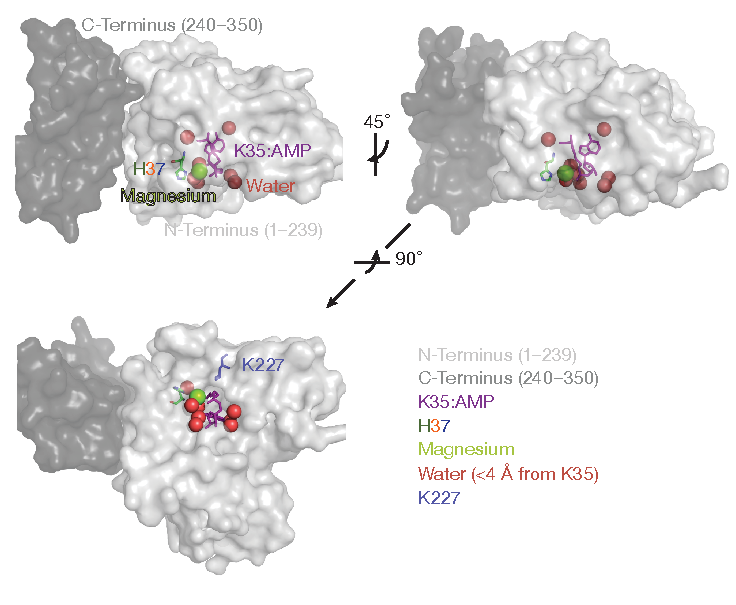
\includegraphics{Figures/Intro/Rnl2_Structure.eps}
      \caption[Structure and active site of pre-adenylated of Rnl2]
      {
        Structure and active site of pre-adenylated of Rnl2\\[0.25cm]
        Rnl2 as crystalized and described by \citep{Nandakumar2006}. Structures from PDB:2HVQ were generated with PyMol. Top left) Rnl2 is composed of a C-terminal and N-terminal domain. Top Right) The active site of Rnl2 is highlighted. Bottom left) Active site of Rnl2 as shown from bottom. This face interacts with substrate. Residue numbering refers to that of the crystal structure.
        }
      \label{Intro:fig:Rnl2 General Structure}
      \end{figure}

    Mutational analysis of Rnl2, and later a crystal structure of the enzyme, have identified key functional residues \citep{Ho2004, Nandakumar2006,Nandakumar2004a,Yin2003d}. The lysine residue at position 35 (K35) receives the AMP in Step 1. The K227 residue in the C-terminal domain is essential for both forward and reverse adenylation of the 5\textprime~PO$_4$ at the nick \citep{Viollet2011}. Mutation of H37 results in an \textasciitilde102 reduced ligation rate, and therefore indicates the essential nature of this residue. Finally, T39 has been shown to interact with the 2\textprime~OH on the 3\textprime~side of the nick, preferring a C3\textprime~endo sugar pucker conformation (see Figure \ref{Intro:fig:Rnl2 Active Site Residues}). Rnl2 has a minimal footprint of 13 nt, centered on the nick, and only requires magnesium for transfer of AMP to the 5\textprime~phosphate. Work done in the Shuman lab \citep{Nandakumar2006} observed that 2\textprime~deoxyribose residues on the 5\textprime~side of the nick (i.e. DNA) adopt an RNA-like sugar pucker, leading to the correct orientation of the 3\textprime~OH relative to the AMP leaving group and resulting in ligation. This conformation is of particular importance to results presented in Chapters \ref{SeqZipPaper} and \ref{SeqZipMethod}.

    \begin{figure} % Rnl2 Active site residues
      \centering 
      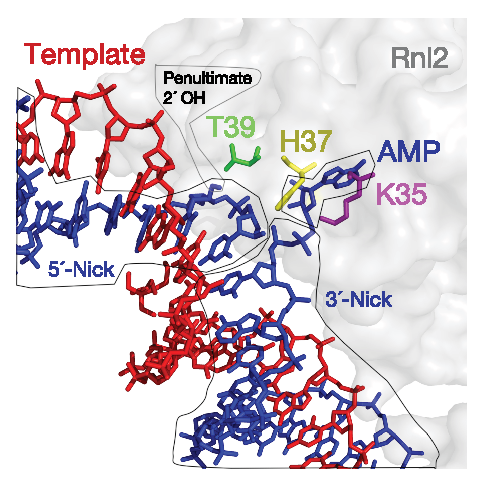
\includegraphics{Figures/Intro/Rnl2_Active_Site_Residues.eps}
      \caption[Active site of T4 RNA Ligase 2 with highlighted residues]
      {
        Active site of T4 RNA Ligase 2 with highlighted residues\\[0.25cm]
        Rnl2 complexed with nicked dsDNA as crystalized and described by \citep{Nandakumar2006}. Structures from PDB:2HVR and generated with PyMol.
        }
      \label{Intro:fig:Rnl2 Active Site Residues}
      \end{figure}

    While Rnl2 is extremely efficient at high concentration, displaying little or no reversible chemistry, a modified version of the enzyme containing only the N-terminal domain and a K227A point mutation (“Truncated mutant”) has no adenyltransferase activity. In this case, adenyltransferase refers to the ligase transferring AMP from an adenylated substrate to itself; reverse chemistry of step 2 in Figure \ref{Intro:fig:Ligation Mechanism}). This mutant has been used in specialized cloning applications \citep{Ghildiyal2008, Hafner2008a, Viollet2011} that take advantage of this activity. In these reactions, the use of pre-adenylated 3\textprime~DNA adaptors allows for selective ligation among already phosphorylated species by limiting the enzyme-catalyzed transfer of AMP from the adaptor to other phosphorylated species. Use of this truncated mutant to create a hybrid RNA/DNA molecule has greatly improved many high-throughput sequencing work flows.

    Ligation of hybrid substrates (eg. DNA-templated RNA:DNA vs DNA-templated DNA:DNA) have revealed general substrate preferences. DNA ligases appear to prefer the residue bearing the 5\textprime~phosphate on the 3\textprime~side of the nick to be 2\textprime~deoxyribose, and have a relaxed requirement for the sugar on the 5\textprime~side of the nick. RNA ligases have the reverse preference, demonstrating higher activities when the 5\textprime~strand, 3\textprime~OH residue also bears a 2\textprime OH. Rnl2 has an additional preference for an RNA residue at the penultimate 3\textprime~side of a nick \citep{Ho2002b,Ho2004, Nandakumar2004a, Nandakumar2006}. The two base requirement for RNA at the 5\textprime~side of the double stranded nick biases Rnl2 to join RNA:[RNA/DNA] strands. Independent labs have measured this preference and have reported that the RNA-templated DNA:DNA joining activity of Rnl2 is below assay limits of detection \citep{Bullard2006}. However, results discussed in this work clearly show that with enough enzyme and sensitive downstream measurements, Rnl2 will catalyze RNA-templated DNA:DNA ligation (see Chapters \ref{SeqZipPaper} and \ref{SeqZipMethod}. Previous reports of Rnl2 lacking this activity are likely due to a single turnover mechanism in this reaction imposed by a non-natural sugar pucker of the ligated DNA kinetically trapping the enzyme on the ligated duplex.

  \subsection{Ligases as molecular tools}

    This section describes the identification and development of ligases as tools in molecular biology. Ligation of templated duplexes has multiple uses in cloning and sequence characterization. The following section (\ref{Intro:sec:Nucleic Acid Polymers}) discusses long nucleic acid polymers, specifically mammalian piRNA precursor transcripts. Little biology is known concerning these long transcripts. Chapters \ref{SeqZipPaper} and \ref{SeqZipMethod} discuss the application of Rnl2 to characterization of long nucleic acid polymers. The final section of this chapter {\ref{Intro:sec:Unique Time in Omics} discusses what is in effect \textit{in silico} ligation of sequence reads--~ Assembly of full-length transcripts from short reads.

\section{Nucleic Acid Polymers}
  \label{Intro:sec:Nucleic Acid Polymers}

  \citet{Fire1998} brought small RNAs to the forefront of research. Recently, lncRNAs has been an exciting area of research \citep{Khalil2009,Guttman2009}. Whether ``small'' or ``long'' all classes of RNA are polymers of ribonucleotides. This section will focus on an interesting class of nucleic acid polymer---Mammalian piRNA precursor transcripts. These transcripts, which share similarities to traditional mRNAs, are eventually processed down to another very interesting class of ``small'' RNA-- mammalian piRNAs. Finally, the section ends with a history of transcript assembly of HTS data, without which the study of both types of polymer would not be possible.

  \subsection{It Started Small: Mammalian piRNAs}
  
    piRNAs are small RNAs 24-- 31 nt long. They are longer than other small RNAs (eg. miRNAs or siRNAs) and are believed to derive from single-stranded RNA precursors because unlike other small RNAs, their biogenesis does not the require double-stranded RNA-specific ribonuclease Dicer \citep{Vagin2006, Houwing2007}. Yet, similar to other small RNAs, they bind a sub group of the Argonaute family of proteins, PIWI proteins, from which their name is derived (\textit{PIWI Interacting RNAs}). 

    \citet{Aravin2001} first identified piRNAs in \flies{} via northern blot probes from the \textit{Su(Ste)} locus as heterogeneoous 25--27 RNAs essential for silencing of \textit{Stellate} and more importantly---male fertility. In the years since the initial report, piRNAs have been catalogued, characterized, manipulated and mutated. Yet, very little about what they do is known. What is known is that without a functioning piRNA pathway male mice are also sterile \citep{Deng2002c,Kuramochi-Miyagawa2004}. Also, studies in humans have correlated SNPs in human PIWI proteins and decreased fertility \citep{Gu2010a}. What is unknown includes: biogenesis of initial transcript to small RNA, physiological targets, and terminal function of sterility maintenance. Especially little is known concerning mammalian piRNAs, on which the following section will focus.

    Virtually all of the what is known concerning piRNA biogensis is infered from flies to other species, including mice \citep{Siomi2011,Luteijn2013,Hirose2014}. Where the parallels break down is what is known concerning \textit{function}. The most famous function for piRNAs in \flies{} is suppression of transposon transcripts during gameotogensis \citep{Malone2009}. The Ping-Pong model elegantly explains how this might be accomplished: cyclic cleavage of transposon transcripts and piRNA precursor transcripts \citep{Brennecke2007,Gunawardane2007}. Yet for mammals, it appears that piRNAs have diversified beyond just transposon silencing.

    Four reports in 2006 defined the beginning of mammalian piRNA research \citep{Aravin2006,Grivna2006,Girard2006,Lau2006}. Each observed small RNA species, most \textasciitilde30 nt long, that bound PIWI proteins. They also noticed that when aligned to the mouse genome, most of the piRNAs clustered in discrete genomic loci. Overtime, it became clear that mammalian piRNAs can divided into three major classes (see Figure \ref{Intro:fig:Mammalian piRNA classes}. There are also three PIWI proteins in mice, each displaying a distinct expression profile during development and an association with piRNAs of a specific length. 

   \begin{figure} % Mammalian piRNA classes
      \centering 
      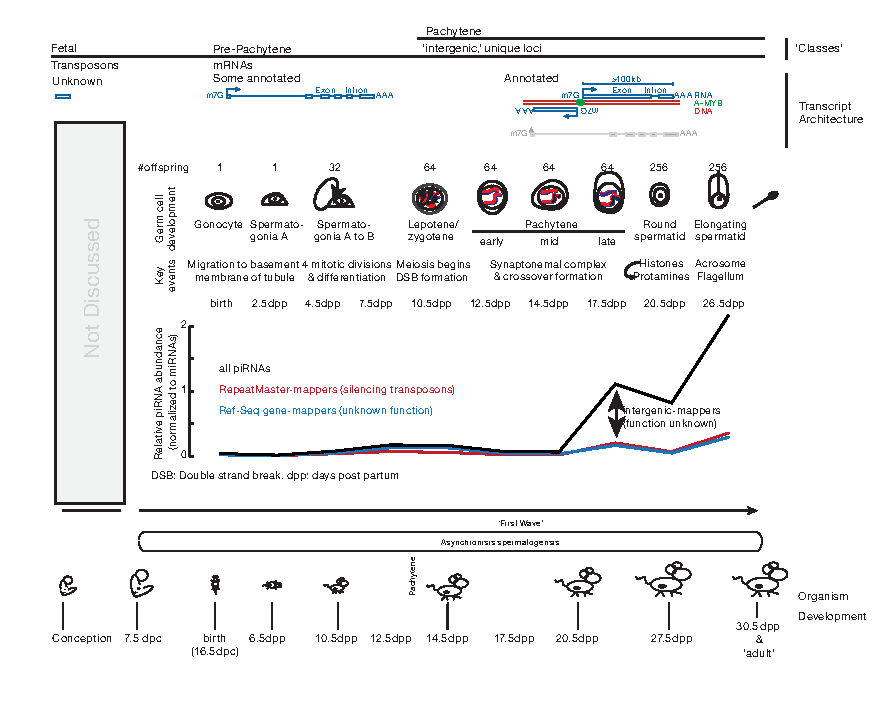
\includegraphics{Figures/Intro/MammalianPiRNAClassesOverTime.eps}
      \caption[Different Classes of mammalian piRNAs]
      {
        Overall view of the three classes of mammalian piRNAs. Figure design assisted by \href{mailto:xin.li@umassmed.edu}{Xin Zhiguo Li}.
        } \label{Intro:fig:Mammalian piRNA classes}
      \end{figure}

    \textit{Fetal piRNAs} are present before birth. These piRNAs tend to be short, bind the PIWI protein MIWI2 (PIWIL4) in mice, and have sequences found in transposable elements \citep{Carmell2007}. Quickly following MIWI2 in expression is the second PIWI protein expressed MILI (PIWIL2). It is during the ``fetal'' stage of piRNA biogenesis in mice that MIWI2 and MILI undergo ping-pong amplification, similar to that observed in flies, in order to silence expression of transposons during germ line formation  \citep{Kuramochi-Miyagawa2004, Aravin2006, Aravin2008a}.

    The next class of piRNAs, historically but confusing grouped with the previous class, are called \textit{Pre-pachytene piRNAs}. Pre-pachytene piRNAs are expressed just before birth and continue to be expressed in functioning testes. These piRNAs tend to map to traditional, annotated, protein-coding genes. After birth, and during the ``neonatal stage'' only MILI is expressed, and piRNAs shift from mostly transposon-mapping to 3\textprime~UTR mapping \citep{Robine2009}.

    Finally, due to their unique sequence in the genome, the genetic origin of millions of piRNAs belonging to the third class, the \textit{pachytene piRNAs}, was immediately known. Once the ``first wave'' of spermatogenesis \citep{Oakberg1956b, Laiho2013a} reaches meiosis, pachytene piRNAs are expressed \citep{Girard2006, Lau2006, Li2013h}. Pachytene piRNAs are extremely abundant after the pachytene stage of meiosis I when chromosomes pair up, cross over, and exchange genetic material. They bind another Piwi protein MIWI (PIWIL1). The genomic origin of pachytene piRNAs, often unique in terms of genomic sequence, map within ``gene deserts''---unannotated and devoid of introns. This is comparable to piRNA clusters in flies, such as \textit{flamenco}, whose transcription can be abolished with a P-element insertion into a putative promoter, as measured by northern blot looking for piRNAs generated 168 kb downstream (see Figure \ref{Intro:fig:flamenco} \citep{Brennecke2007,Goriaux2014}. This gene architecture makes the pachytene piRNA loci some of the most interesting RNA-producing regions of the mammalian genome. These clusters, (aka: ``piRNA-producing loci'' or ``genes'') appear to produce a single, continuous, relatively long, and un-spliced Pol II transcript \citep{Li2013h}. 

    \begin{figure} % Flemenco Locus
      \centering 
      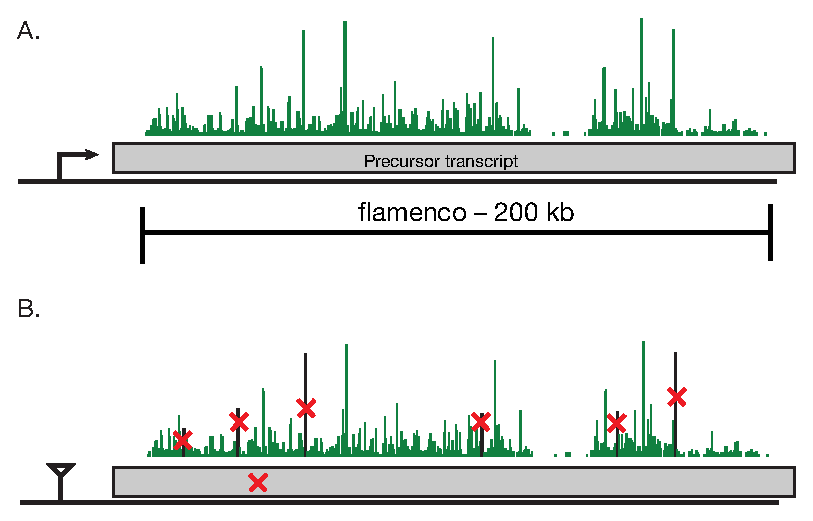
\includegraphics{Figures/Intro/FlamencoLocus.eps}
      \caption[Genetic evidence for long, continuous fly piRNA precursor transcripts]
      {
        A the \flies{} gene \textit{flamenco} is a graveyard for transposon sequences \citep{Pelisson1994}. Evidence for expression of a single-contiguous RNA transcript from \textit{flamenco} (A) is provided by a P-element insertion into the suspected promoter region (B). \citep{Brennecke2007} could not detect specific piRNAs (red X's) by northern blot in the P-element mutant.
        }
      \label{Intro:fig:flamenco}
      \end{figure}

  \subsection{From Long to Small: Precursor processing to mature piRNAs}
    \label{Intro:subsec:Processing of piRNAs in mice}

    The process by which a long, single-stranded piRNA precursor transcript becomes a small mature piRNA is full of black boxes and question marks. While we do know they are long, single-stranded piRNA transcripts \citep{Brennecke2007,Li2013e}, we are very unsure of many of the steps between transcription and terminal function of piRNA::PIWI complexes (PIWI-piRISC).

    For example: How do piRNA precursor transcripts exit the nucleus? This is not known in mice, but there are clues in \flies{}, where some piRNA clusters are bidirectionally transcribed and bound by the HP1 homologue Rhino \citep{Klattenhoff2009}. Rhino co-localizes with the DEAD box protein UAP56 near the perinuclear compartment known as nuage \citep{Zhang2012}. It is believed that Rhino and UAP56 assist in a handoff of large precursor transcripts across the nuclear envelope where they are bound by the nuage-protein VASA \citep{Zhang2012}.

    Once precursor transcripts exit the nuclease they likely enter chromatoid bodies (comparable to nuage in flies) \citep{Lim2007,Meikar2011,Zhang2012}. There they are then believed to be ``Fragmented'' into shorter \textit{piRNA intermediates} \citep{Saito2010,Li2013} by the protein MitoPLD (aka: PLD6) \citep{Watanabe2011a}. Structures of the fly homologue of MitoPLD, \textit{Zucchini}, supports slicing activity in vitro \citep{Nishimasu2012,Ipsaro2012}, but this activity has yet to be shown in vivo \citep{Luteijn2013}. Fragmentation may, or may not, impart the 5\textprime~U preference seen in mature piRNAs \citep{Gunawardane2007,Brennecke2007} and indeed Zucchini does not show a 5\textprime~U bias in vitro \citep{Nishimasu2012,Ipsaro2012}. However, this preference may result from downstream sequence preference of PIWI-protein binding \citep{Cora2014}.

    Once fragmented into shorter RNAs, piRNA intermediates seem to be ``Loaded,'' into a specific time- and expression-appropriate PIWI protein (see Figure \ref{Intro:fig:Mammalian piRNA classes}). Following ``Loading,'' piRNA intermediates are trimmed down to the length characterstic of bound Piwi by the appropriately named, but \textit{hypothetical}, enzyme ``TRIMMER'' \citep{Kawaoka2011}}. Both ``Loading'' and ``Trimmer'' activity have not been shown in mammalian systems, but inferred from Silk worm (\textit{Bombyx mori}) cellular extracts of ovary-derived BmN4 cells \citep{Kawaoka2009}. Once trimmed, piRNAs are methylated on the 2\textprime~OH position by the enzyme HEN1 \citep{Horwich2007,Kirino2007,Kawaoka2011}. At this point, a mature piRNA, complexed with a PIWI protein (PIWI-piRISC), is poised to perform its intended cellular function.

    \begin{figure}\small % Mammalian piRNA Pathway
     \centering 
     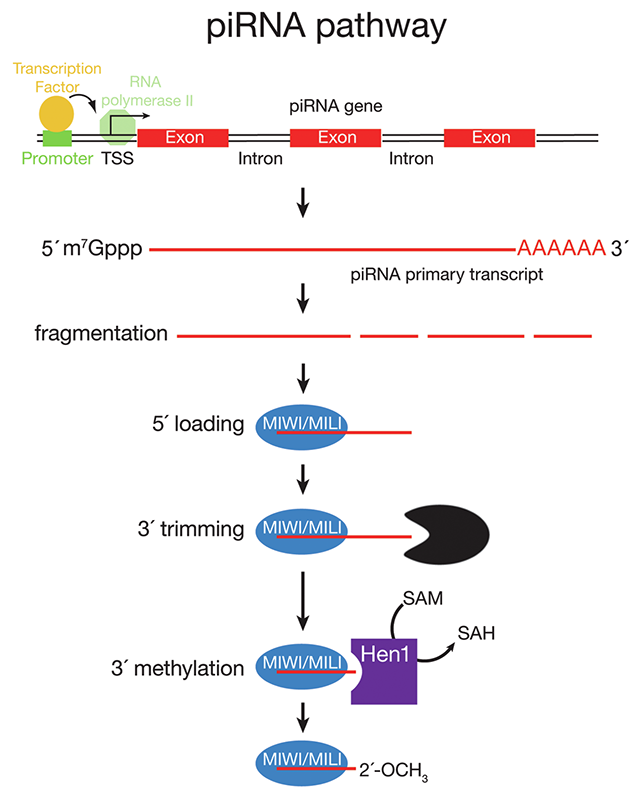
\includegraphics{Figures/Intro/mammalian_piRNA_pathway.png}
     \caption[A model for Mammalian piRNA biogenesis]
     {
       Figure taken from \citep{Li2013e}: A model for piRNA biogenesis. Primary piRNA transcripts are transcribed by RNA polymerase II and contain 5\textprime~caps, exons and introns and poly(A) tails. The transcription of pachytene piRNA genes is controlled by A-MYB; transcription factor(s) (TF) controlling pre-pachytene piRNA genes remain to be discovered. Current models of piRNA biogenesis propose that PLD6 determines the 5\textprime~end of piRNA intermediates with lengths >30 nt. These intermediates are proposed to then be loaded into PIWI proteins. After PIWI binding, a nuclease is thought to trim the 3\textprime~end of the piRNA to the length characteristic of the particular bound PIWI protein. Finally, further trimming is prevented by addition of a 2\textprime~-O-methyl group to the 3\textprime~end of the mature piRNA by the S-adenosylmethionine-dependent methyltransferase HEN1. Figure adapted from \citep{Li2013}.
       }
     \label{Intro:fig:Mammalian piRNA BioGensis}
     \end{figure}

    Once loaded, what are the cellular activities of PIWI-piRISC? MILI and MIWI2 have been shown to direct epigenetic LINE1 and IAP transposon silencing in the embryonic male germline \citep{Aravin2007,Carmell2007,Kuramochi-Miyagawa2008}. Two studies \citep{DeFazio2011,Reuter2011} used point mutations in the catalytic triad of MIWI, MIWI2, and MILI to remove slicer activities. \citet{DeFazio2011} found that MIWI2 deficient mice are fertile, silence transposons, and display all signs of secondary piRNA biogensis and concluded that MILI (which were sterile) was required for transposon silencing. \citet{Reuter2011} focused on MIWI and found that it required for silencing of LINE1 transcripts long after they were epigentically silenced (i.e. in the adolecent mouse).

    The above studies point to a familiar scenario of piRNA-mediated target cleavage and/or transcriptional silencing by PIWI-piRISC \citep{Meister2013}. 
    
    Yet confusingly, HITS-CLIP of MIWI revealed that MIWI binds spermiogenic mRNAs without a piRNA guide \citep{Vourekas2012} and \citet{Reuter2011} demonstrated that slicing of target by MIWI RISC requires near perfect binding.
    
    How does does one reconcile these findings with the extremely uniquely-mapping quality of virtually all pachytene piRNAs? Put another way, if MIWI requires near perfect pairing between guide and target, and pachytene piRNAs perfectly pair with nothing else in the genome but antisense transcripts from their own loci, what is the mechanism taget recognition? In fact, when taking all studies on the function of mouse piRNAs, frustratingly little is actually known, or internally consistent. This is in stark contrast to interactions between other Argonaute proteins in the siRNA or miRNA pathways. Indeed, the catalytic nature of PIWI proteins is a debated topic \citep{Luteijn2013,Meister2013}.

    Perhaps the site of PIWI-piRISC function is not cytoplasim. Indeed, fly PIWI is localized in the nucleus, and MILI and MIWI2 have been shown in induce DNA methylation \citep{Cox2000,Aravin2008}. This is a potentially misleading course of logic. Localization does not confirm interaction \citep{North2006}, or function and infering such from localization can be as dangerous as assuming cars function in parking lots. Finally, a extremely tantalizing additional potential function for mammalian piRNAs is that of genomic imprinting \citep{Watanabe2011}. This function is in good agreement with germline-specific and developmentally timed nature of Piwi protein expression.

    In summary, there are still many holes and black boxes in the story of mammalian piRNAs. Continued study is easily justified by the sterile phenotypes of all pathway mutants. Time will tell if mammalian piRNAs are involving in a satisfying process of biology or are crude side quest of Nature.


  \subsection{From Short to Long: Transcript Assembly}
    \label{Intro:subsec:Tx Assembly}

    Initial genome-wide HTS of piRNAs revealed a tremedous amount of biology \citep{Gunawardane2007,Brennecke2007}, but could provide very little information as to the original transcriptional unit. The ability to reconstruct piRNA precursors had to wait for technological improvements in HTS read length and alignment algorithms.

    Working backwards from small RNA-Seq data to original transcription units was impossible. Mammalian piRNAs are too short (\textasciitilde30 nt) to allow for quality assembly using even the most current algorithms. They simply do not provide the necessary overlap of sequence to build scaffolds. Also, repeat elements are extremely abundant in mice \citep{Nellaker2012}, and combined with short reads, furthur reduce the abilty to assemble full-length sequences. Therefore, it was necessary sequence RNAs prior to mature piRNA formation.

    Even with longer read lengths and the best alignment algorithms, the 5\textprime~ and 3\textprime~ ends of long and diverse transcripts like piRNA precursors often requires a combination of multiple HTS datatypes \citep{Blower2013}. Tailored versions of RNA-Seq, such as CAP-Seq (see section \ref{Intro:subsec: History of HTS}), are not sufficient for accurate 5\textprime~ end determination, and require orthogonal datasets to verify TSSs. Taking a page from lncRNA transcript discovery, orthogonal data such as ChIP-Seq of H3K4 methylated histones, a marker for transcriptional initiation \citep{Khalil2009}. More information about how multiple HTS datasets can be, and were used, to define the transcriptional unit of piRNA precursors transcripts is provided in Chapter \ref{MolCel}.

    General assembly of full length transcripts (not just piRNA precursor transcripts) is difficult for at least 3 reasons. 1) The transcriptome is expressed across 5 orders of magnitude and a typical RNA-Seq library containing many reads from a few highly-expressed genes, and many fewer reads from lowly-expressed genes \citep{Blencowe2009}; 2) RNA-Seq libraries are often not created from a completely pure source of mRNA and can contain reads from other RNA classes (e.g. tRNAs) or intronic reads from pre-mRNAs; and 3) Reads are often much shorter than a typical mRNA, making it difficult to assign which read goes to which isoform of a given gene (see the ``connectivity problem'' discussed in section \ref{Intro:sec:Isoform Problem}. With these challenges in mind, what is the current state of transcript reconsuction (herein transcript assembly)?

    Computational transcriptome assembly of short reads is currently performed in one of two modes: genome-guided and genome-independent \citep{Garber2011a}. The difference between these two approaches is use of a high-quality genome during the reconsruction process. Popular assembly programs such as Cufflinks \citep{Trapnell2010} and Scripture \citep{Guttman2010}, use genome-aligned short reads as the bases for calling transcripts.

    As mentioned previously, constraints imposed by the huge dynamic range of RNA expression is the major complicating factor with current transcript assembly programs. These programs frequently generate short transcript fragments, or contigs, due to poor coverage on long and lowly-expressed transcripts \citep{Rehrauer2013}. Merging these contigs into a continuous annotation is a major goal. Improvements will surely come from greater sequencing depth, longer reads, and mRNA enrichment schemes, albiet with dimishing returns \citep{Chang2014c}. Longer-term barriers include repetive sequences, transcript secondary structure \citep{Wan2014}, and mRNA processing including hydrolysis and RT processivity \citep{Sharon2013}. Finally, multiple forms of mRNA enrichment and purification, specifically combining poly(A)+ tail and 5\textprime~CAP selection, can be used to increase the accuracy of mRNA transcript assembly \citep{Blower2013}. 

\section{A unique time in ``'omics''}
  \label{Intro:sec:Unique Time in Omics}

  Biomedical science has just taken the first few steps into a new era. Most questions, including those of gene expression, molecular interactions, and evolution should no longer be asked on a small scale. Indeed questions and hypothesis concerning these topics should be approached on a ``big scale'' from the very onset, in order to maximize return on investment. Much of the work required to reap maximum benefit falls squarely on our own education and experience. See section \ref{Disc:sec:Final Thoughts} for concluding thoughts.


